% !TEX root = ../main.tex
\pagebreak[0]
\section{Reduction to exact arithmetic}\label{sec:reduction-to-exact-arithmetic}

The Domain component reduces its whole-box test to finitely many sign
comparisons in $\mathbb Q(\sqrt5)$. We explain how to perform these
comparisons using integers, then develop a sign test for the polynomial
inequalities needed by the geometric components.

For a general polynomial, negative values at the midpoint, or even at
every corner, do not establish negativity throughout a box. The Domain
component's corner criterion relies on the particular affine and concave
expressions in its proof. To handle more general expressions, we write a
polynomial on a box as a weighted average of finitely many numbers, its
Bernstein coefficients, which can be computed exactly. When all of them
are negative, so is the polynomial throughout the box, including its
boundary. Every elimination in this article that is not a direct endpoint
comparison ends in this single test.

\subsection{Exact representation of field elements with integers}\label{subsec:exact-representation-of-field-elements-with-integers}

The standard arithmetic of $\mathbb Q(\sqrt5)$ gives exact field operations
and sign and equality tests using only integer calculations.
As introduced in \cref{subsec:parametrisation-of-the-configuration-space},
we represent $a+b\sqrt5$ by the rational pair $(a,b)$, storing each rational
number as a ratio of arbitrary-size integers with positive denominator.
The operations are as follows:
\begin{itemize}
  \item \emph{Addition and subtraction} act componentwise on the pairs.
  \item \emph{Multiplication} uses
    \[
      (a+b\sqrt5)(a'+b'\sqrt5)
        =(aa'+5bb')+(ab'+ba')\sqrt5.
    \]
  \item \emph{Division} uses the reciprocal of a nonzero field element:
    \[
      \frac{1}{a+b\sqrt5}=\frac{a-b\sqrt5}{a^2-5b^2}.
    \]
    The denominator cannot vanish unless $a=b=0$, since $\sqrt5$ is irrational.
  \item \emph{Equality and sign comparisons} are exact. An element is zero
    exactly when $a=b=0$. If either coefficient is zero, or both have the
    same sign, the sign of $a+b\sqrt5$ is immediate. If their signs differ,
    compare the rational squares $a^2$ and $5b^2$:
    \[
      \operatorname{sign}(a+b\sqrt5)
        =\operatorname{sign}(a)\,
          \operatorname{sign}(a^2-5b^2).
    \]
    The preliminary sign distinction is essential before using this squared
    comparison. Comparing two field elements reduces to testing their difference.
\end{itemize}
These operations supply the exact comparisons required by the tests of the
Domain component in \cref{subsec:domain-component-skipping-boxes-outside-the-reduced-domain}.

\subsection{Bernstein coefficients}\label{subsec:bernstein-coefficients}

To eliminate a box, a component must show that some polynomial is strictly
negative at every point of the box, not only at finitely many sampled
configurations. We use a classical tool for this
\citep[Section~3]{Garloff1986}. Consider first a
polynomial $p$ of degree at most $n$ in one variable $x$ on an interval
$[l,h]$ of width $w=h-l\ge0$. Substituting $x=l+wy$ gives a polynomial in
$y\in[0,1]$, which can be written uniquely as
\begin{equation}\label{eq:one-variable-bernstein-form}
  p(l+wy)=\sum_{k=0}^{n}b_k\binom nk y^k(1-y)^{n-k}.
\end{equation}
The numbers $b_k$ are the \emph{Bernstein coefficients} of $p$ on $[l,h]$.
The $n+1$ polynomials $\binom nk y^k(1-y)^{n-k}$ are nonnegative on
$[0,1]$, and by the binomial theorem they add up to
${(y+(1-y))}^n=1$. Every value of $p$ on the interval is therefore a
weighted average of its Bernstein coefficients, and if all of them are
negative, so is $p$.

\paragraph{A worked example.}
The polynomial $p(x)=-1+3x-3x^2$ is negative on $[0,1]$: its largest
value there is $p(1/2)=-1/4$. Its Bernstein coefficients on $[0,1]$ are
$(-1,1/2,-1)$, so the test does not yet succeed. After halving, the
coefficients are $(-1,-1/4,-1/4)$ on $[0,1/2]$, where
$p(y/2)=-1+\tfrac32y-\tfrac34y^2$, and $(-1/4,-1/4,-1)$ on $[1/2,1]$.
Both halves pass. This is typical: halving brings the coefficients closer
to the values of the polynomial, as we make precise below.

\begin{figure}[htbp]
\centering
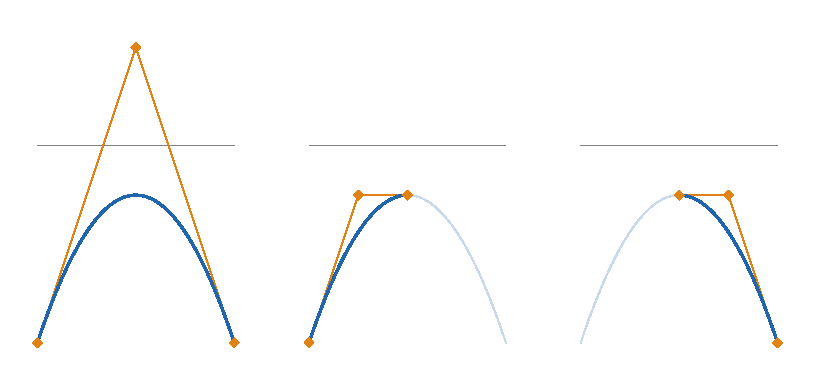
\includegraphics[width=0.85\linewidth]{figures/bernstein}
\caption{\fc{Plug}{The polynomial $p(x)=-1+3x-3x^2$ (blue)}, \fc{Hole}{its Bernstein coefficients (orange diamonds, at $x=l+k(h-l)/2$) and their control polygon}; \fc{Grey}{grey is the axis $p=0$}. Left: on $[0,1]$ the middle coefficient is positive although $p$ is negative throughout, and the sign test refuses. Middle and right: on the two halves, shown with the whole graph for reference, every coefficient is negative and the test succeeds. On each interval the graph lies between the smallest and the largest coefficient.}
\label{fig:bernstein-example}
\end{figure}

\paragraph{Several variables.}
Let $p$ be a polynomial in $x_1,\dots,x_k$ with coefficients in
$\mathbb Q(\sqrt5)$, of degree $n_j$ in $x_j$, and let
$B=\prod_j[l_j,h_j]$ be a closed box with rational endpoints and widths
$w_j=h_j-l_j\ge0$. With $x_j=l_j+w_jy_j$, the products
\[
  B_{\mathbf i}(\mathbf y)=\prod_{j=1}^{k}\binom{n_j}{i_j}
      y_j^{i_j}{(1-y_j)}^{n_j-i_j},
  \qquad 0\le i_j\le n_j,
\]
form a basis of the polynomials of degree at most $n_j$ in each $y_j$.
The unique coefficients $b_{\mathbf i}$ with
\[
  p(l_1+w_1y_1,\dots,l_k+w_ky_k)=\sum_{\mathbf i}b_{\mathbf i}B_{\mathbf i}(\mathbf y)
\]
are the \emph{tensor Bernstein coefficients} of $p$ on $B$; there are
$\prod_j(n_j+1)$ of them.

\begin{lemma}[Bernstein sign test]\label{lem:bernstein-sign-test}
  If every tensor Bernstein coefficient of $p$ on $B$ is strictly
  negative, then $p(\mathbf x)<0$ for every $\mathbf x\in B$.
\end{lemma}
\begin{proof}
  Each $B_{\mathbf i}$ is nonnegative on ${[0,1]}^k$, and their sum is
  $\prod_j{(y_j+(1-y_j))}^{n_j}=1$. A point $\mathbf x\in B$ corresponds to
  $y_j=(x_j-l_j)/w_j$, or to any $y_j\in[0,1]$ when $w_j=0$. So
  $p(\mathbf x)$ is a convex combination of the coefficients and at most
  their maximum, which is negative. This covers every real point of the
  closed box, including its faces and corners and points with irrational
  coordinates.
\end{proof}

The coefficient with every $i_j\in\{0,n_j\}$ is the value of $p$ at the
corresponding corner of $B$. The test therefore refuses a polynomial that
is nonnegative at some corner, and more generally anywhere in $B$. For a
polynomial of degree at most one in each variable, the coefficients are
exactly its corner values, so the test coincides with the endpoint rule of
the Domain component in
\cref{subsec:domain-component-skipping-boxes-outside-the-reduced-domain}.
A refusal never proves anything: it only leaves the box unresolved.

\paragraph{Exact computation.}
The coefficients are computed one variable at a time. Fix $j$, write
$n=n_j$, and expand along $y=y_j$ as
$p=\sum_ka_ky^k$, with coefficients that are polynomials in the other
variables. The identity
\[
  y^k=\sum_{r=k}^{n}\frac{\binom rk}{\binom nk}\binom nr y^r{(1-y)}^{n-r}
\]
converts powers of $y$ into the Bernstein basis, giving
\begin{equation}\label{eq:bernstein-from-power-coefficients}
  b_r=\sum_{k=0}^{r}\frac{\binom rk}{\binom nk}a_k .
\end{equation}
Substitution, expansion and this change of basis use only exact field
operations in $\mathbb Q(\sqrt5)$. In practice we first multiply by a
common denominator, so that every step is an operation on integers of
$\mathbb Z[\sqrt5]$ followed by a known positive scale, and read the sign
of each coefficient with the exact test of
\cref{subsec:exact-representation-of-field-elements-with-integers}.

\paragraph{Convergence under subdivision.}
Refinement helps wherever a polynomial is strictly negative, because the
coefficients approach the values of the polynomial as the box shrinks.

\begin{lemma}[Convergence of Bernstein coefficients]\label{lem:convergence-of-bernstein-coefficients}
  Let $p$ be a polynomial and $K$ a bounded box. There is a constant $C$
  such that for every box $B\subseteq K$ whose widths are all at most
  $w\le1$, every tensor Bernstein coefficient of $p$ on $B$ differs from
  the value of $p$ at the lower corner of $B$ by at most $Cw$. In
  particular, if $p<0$ throughout a closed box $B_*$, every box
  $B\subseteq B_*$ with sufficiently small widths passes the test of
  \cref{lem:bernstein-sign-test}.
\end{lemma}
\begin{proof}
  In one variable, $a_0=p(l)$ and $a_k=p^{(k)}(l)w^k/k!$ by Taylor's
  formula. In \cref{eq:bernstein-from-power-coefficients}, every weight
  lies in $[0,1]$ and the weight of $a_0$ is one, so
  \[
    |b_r-p(l)|\le\sum_{k\ge1}|a_k|
      \le w\sum_{k\ge1}\frac{|p^{(k)}(l)|}{k!}.
  \]
  The derivatives are bounded on $K$. Converting one variable at a time
  applies this bound to polynomials whose coefficients are themselves
  bounded on $K$, and the errors add, giving the constant $C$. For the
  second claim, $p\le-\gamma$ on $B_*$ for some $\gamma>0$ by compactness;
  every coefficient on a subbox of widths at most $w<\gamma/C$ is then at
  most $-\gamma+Cw<0$.
\end{proof}

On a search box, every polynomial we test has degree at most two in each
of the five parameters, so a test inspects at most $3^5=243$ coefficients.
The same test applies after a polynomial change of variables, which is how
the later components use it, through the zoom lemma of
\cref{subsec:the-zoom-lemma}.
